\documentclass[preprint,12pt,authoryear]{elsarticle}

\usepackage[T1]{fontenc}
\usepackage{lmodern}
\usepackage{amsmath,amssymb}
\usepackage{booktabs}
\usepackage{array}
\usepackage{threeparttable}
\usepackage{graphicx}
\usepackage{setspace}
\usepackage{lineno}
\usepackage[hidelinks]{hyperref}
\usepackage[margin=1in]{geometry}

\onehalfspacing
\linenumbers
\journal{Finance Research Open}

\newcommand{\tablenote}[1]{\par\vspace{0.4em}\begin{minipage}{\linewidth}\footnotesize #1\end{minipage}}

\begin{document}

\begin{frontmatter}

\title{Execution-Aware Alpha Mining: Teaching LLM Factor Agents to Account for Trading Costs}

\begin{abstract}
Large language model (LLM) agents are increasingly used to search for formulaic trading signals, but these searches usually score candidates on gross predictive quality and leave trading costs to implementation. We study how cost-awareness inside the search changes what an LLM agent finds. A locally hosted LLM proposes daily cross-sectional equity factors in a constrained expression language; each candidate is backtested on a survivorship-free, point-in-time S\&P 500 universe and priced with a spread-and-impact cost model. Across 21 walk-forward folds (2006--2026), four seed signals and three sampling seeds, we compare three feedback conditions that share one search procedure: a cost-blind reward, a cost-penalized reward presented without explanation, and the same reward accompanied by explicit cost guidance. Cost-blind search settles on 36--103\% daily turnover and loses its entire capital in every category despite positive gross Sharpe ratios. The cost-penalized reward alone raises fold-level net Sharpe by 7.9 points (95\% CI 6.4--9.6), mostly by pulling deeply negative ratios toward zero; explicit guidance adds a further 2.4 (1.3--3.7), cuts turnover to 1.4--3.9\% per day and produces the long-horizon smoothing found in the winning factors. Only the low-volatility seed becomes profitable (net Sharpe 0.51; Fama--French five-factor plus momentum alpha of 7.8\% per year, $t = 3.5$), and there the original signal, smoothed or rebalanced monthly by hand without the LLM, does as well. The objective given to an automated factor search, and how it is communicated to the agent, is therefore a first-order economic design choice.
\end{abstract}

\begin{keyword}
LLM agents \sep alpha mining \sep transaction costs \sep turnover \sep reward design \sep walk-forward backtesting \sep point-in-time universe
\JEL G11 \sep G12 \sep C45 \sep C63
\end{keyword}

\end{frontmatter}

\section{Introduction}\label{sec:intro}

Generative language models are now routinely used as a search process over candidate trading signals: a model proposes a formulaic factor, a backtest scores it, and the loop repeats, in the spirit of automated formulaic-alpha search \citep{kakushadze2016}. In such a loop the reward function is the research objective. When the reward is gross in-sample return quality, the search has every reason to favor short-horizon, high-turnover signals, because fast cross-sectional effects carry attractive raw Sharpe ratios that are largely compensation for the spreads and price impact a trader would pay to capture them \citep{korajczyk2004,novymarx2016}.

A fast-growing literature builds LLM-driven alpha-mining systems. Most of this work improves the search mechanism itself: regularized exploration against alpha decay \citep{tang2025}, trajectory-level evolution \citep{han2026}, chained generation and refinement with backtest feedback \citep{cao2025}, code-level evolutionary search \citep{liu2026} and structured exploration of trading semantics \citep{yi2026}. Multi-objective formulations add temporal stability, perturbation robustness and diversity to predictive power \citep{zhao2026}, and a recent survey lists tradability among the dimensions on which such systems should be evaluated \citep{yu2026}. Closest to our setting, \citet{shi2026} include turnover as one of five equally weighted, percentile-ranked criteria in a Monte Carlo tree search reward and report, through a cumulative ablation, that adding it improves trading metrics. LLM output variability itself also implies turnover and cost in LLM-driven stock selection \citep{chon2025}. What is missing is a controlled answer to two questions: how much does putting an explicit dollar cost model inside the search objective change what an LLM agent finds, and does it matter whether the agent is told what that objective penalizes?

We answer both with a reproducible pipeline. A locally hosted LLM proposes factors in a whitelisted, syntax-validated expression language over daily price and volume data. Each candidate becomes a dollar-neutral long--short portfolio on a survivorship-free point-in-time S\&P 500 universe, is priced with a \citet{corwin2012} spread estimator plus square-root impact, and the resulting diagnostics are returned to the agent each round. We run the identical loop under three feedback conditions. The \emph{cost-blind} arm is rewarded on gross Sharpe ratio. The \emph{reward-only} arm is scored on a cost-penalized reward but sees the cost-blind arm's prompt verbatim, except that its reward is described only as an undisclosed scalar. The \emph{execution-aware} arm receives the same cost-penalized reward together with an explanation of what it penalizes, a turnover target and rule-based critiques that recommend smoothing when turnover is high. Moving from the cost-blind to the reward-only arm isolates the reward as selection pressure; moving from the reward-only to the execution-aware arm isolates the cost-focused language. Every comparison is repeated across four economically distinct seed signals, three LLM sampling seeds and 21 rolling walk-forward folds from 2006 to 2026.

Four findings emerge. First, cost-blind search is destructive: it settles on 36--103\% daily turnover and loses its entire capital in all four categories even though its average gross out-of-sample Sharpe ratio is positive (0.56); in the low-volatility category it degrades a seed signal that breaks even on its own into a net Sharpe ratio of $-3.6$. Second, the cost-penalized reward by itself recovers most of the damage, raising fold-level net Sharpe by 7.9 points (95\% CI 6.4--9.6), about three quarters of the total improvement. This figure and the others below are differences in net Sharpe ratio between arms, not Sharpe ratios of any portfolio: they measure how far each arm lifts the deeply negative cost-blind ratios toward zero. Third, explicit cost guidance adds a further 2.4 (1.3--3.7): it lowers turnover from 2.7--46\% to 1.4--3.9\% per day, makes the search converge on long-window smoothed expressions, and is what keeps the reversal and volume categories from losing their entire capital. Fourth, cost-awareness prevents losses more than it creates alpha. Only the low-volatility seed becomes profitable (net Sharpe 0.51, CAGR 5--6\% over 20.6 years, a Fama--French five-factor plus momentum alpha of 7.8\% per year), and in that category the seed signal, smoothed or rebalanced monthly by hand without the LLM, does as well as the search. The results are insensitive to the penalty weights: all nine alternative weightings we test remain net profitable.

The contribution is a controlled decomposition rather than a new search architecture. Holding the model, sampling seed, search budget, starting expression and data fixed, we show that the specification of an automated search's objective, and how that specification is communicated to an LLM agent, determines whether the search creates or destroys value net of costs. A pipeline that reports a discovered factor's Sharpe ratio without disclosing the objective that produced it leaves the result difficult to interpret.

\section{Data and methodology}\label{sec:method}

\subsection{Universe and data}\label{sec:data}

Point-in-time S\&P 500 membership and daily prices come from the Sharadar Core US Equities bundle \citep{sharadar2026}. Replaying the add and remove events of its constituent table reproduces each of its 114 quarterly constituent snapshots from 1998 to 2026 exactly. Between June 1999 and August 2026 the index had 1,119 distinct constituents, 481 of which were later delisted; all of them keep their full price history, and on every trading day at least 99.6\% of index members have a price. Open, high and low prices are rescaled to the dividend-and-split-adjusted close, and days without trading are treated as missing.

To keep the search computationally tractable, each walk-forward fold trades a liquidity-capped subset of the index: the 150 constituents with the highest trailing two-year average dollar volume, measured only over days on which each stock was a member and only with data available before the selection date. The selection is repeated at the start of each training year and at the start of the test year, so the fold's universe is refreshed annually without look-ahead. The union of a fold's annual selections contains 201--246 names (\ref{app:universe}).

\subsection{Factor language}\label{sec:language}

Candidates are single-line expressions over open, high, low, close, volume and a typical-price proxy, built from a whitelisted set of cross-sectional ranks, time-series ranks and z-scores, linearly decaying moving averages (\texttt{decay\_linear}), simple moving averages, rolling standard deviations and arithmetic. Each expression is parsed with Python's abstract-syntax-tree module and rejected unless every node is whitelisted. Six further rules reject degenerate constructions before any backtest: redundant re-ranking, rescaling by a positive constant, directly nested smoothers, unprotected division, exponents above two and rolling windows outside 2--252 days (\ref{app:guardrails}). Expressions with more than eight operator nodes incur a complexity penalty of 0.05 per extra node in every arm.

\subsection{Portfolio construction and trading costs}\label{sec:costs}

On each day the factor's scores are restricted to the current universe, demeaned across stocks and scaled to a dollar-neutral book with 100\% long and 100\% short exposure. Weights formed from day-$t$ inputs are applied with a one-day lag, so a position earns the close-to-close return from day $t$ to day $t+1$ and no same-day price information enters a backtest. Daily one-way turnover is half the sum of absolute differences between the target weights and the previous day's weights after they have drifted with that day's returns, so passive price drift is not counted as trading (\ref{app:turnover}).

Each trade pays half the \citet{corwin2012} high--low spread estimate, clipped to 1--100 basis points, plus square-root impact $0.5\,\sigma\sqrt{q/\mathrm{ADV}}$, where $\sigma$ is the stock's 21-day return volatility and $q/\mathrm{ADV}$ is the trade's share of 21-day average dollar volume for a \$100 million book \citep{grinold2000}. Net returns subtract this cost on every day's weight changes. As a check on the cost model we also report results under flat one-way costs of 5, 10 and 20 basis points. The full model is deliberately conservative. The \citet{corwin2012} estimate is noisy when true spreads are narrow, and clipping negative estimates up to 1 basis point biases its average upward; for the portfolios studied here the model charges 23--28 basis points per unit traded on average, which is high for the most liquid S\&P 500 stocks. The flat 5-basis-point case is therefore the closer approximation to realistic costs for this universe.

\subsection{Agent loop and the three feedback conditions}\label{sec:arms}

Figure~\ref{fig:arch} summarizes the loop. The agent is Qwen2.5-Coder-14B-Instruct (4-bit Q4\_K\_M quantization) run locally through llama.cpp with temperature 0.7 and nucleus sampling at 0.9. In pilot runs, temperatures of 0 and 0.3 collapsed to a single repeated proposal within two rounds (\ref{app:llm}). Each round the agent receives a fixed system prompt describing the expression language and its rules, the best factor found so far and the most recent proposal with their in-sample diagnostics (gross Sharpe, net Sharpe, turnover, cost drag, drawdown, node count and reward) and a rule-based critique of the most recent proposal. It returns one new expression. Every arm sees the same diagnostics, including turnover and cost; the arms differ only in how candidates are scored and in the text describing the reward and critiquing proposals (Table~\ref{tab:arms}).

The cost-penalized reward is
\begin{equation}
R = \mathrm{SR}_{\mathrm{gross}} - \gamma_1\,\mathrm{TO} - \gamma_2\,\mathrm{CI},
\label{eq:reward}
\end{equation}
where $\mathrm{SR}_{\mathrm{gross}}$ is the annualized gross Sharpe ratio, $\mathrm{TO}$ the annualized one-way turnover (as a multiple of capital) and $\mathrm{CI}$ the annualized cost drag, with $\gamma_1 = 0.5$ and $\gamma_2 = 8$ in the main experiments. The cost-blind reward is $\mathrm{SR}_{\mathrm{gross}}$. The reward-only arm is scored with Eq.~\eqref{eq:reward} but receives the cost-blind arm's prompt and critiques verbatim, except that its reward sentence describes an undisclosed scalar computed from the diagnostics. Section~\ref{sec:gamma} varies $\gamma_1$ and $\gamma_2$.

\begin{figure}[t]
\centering
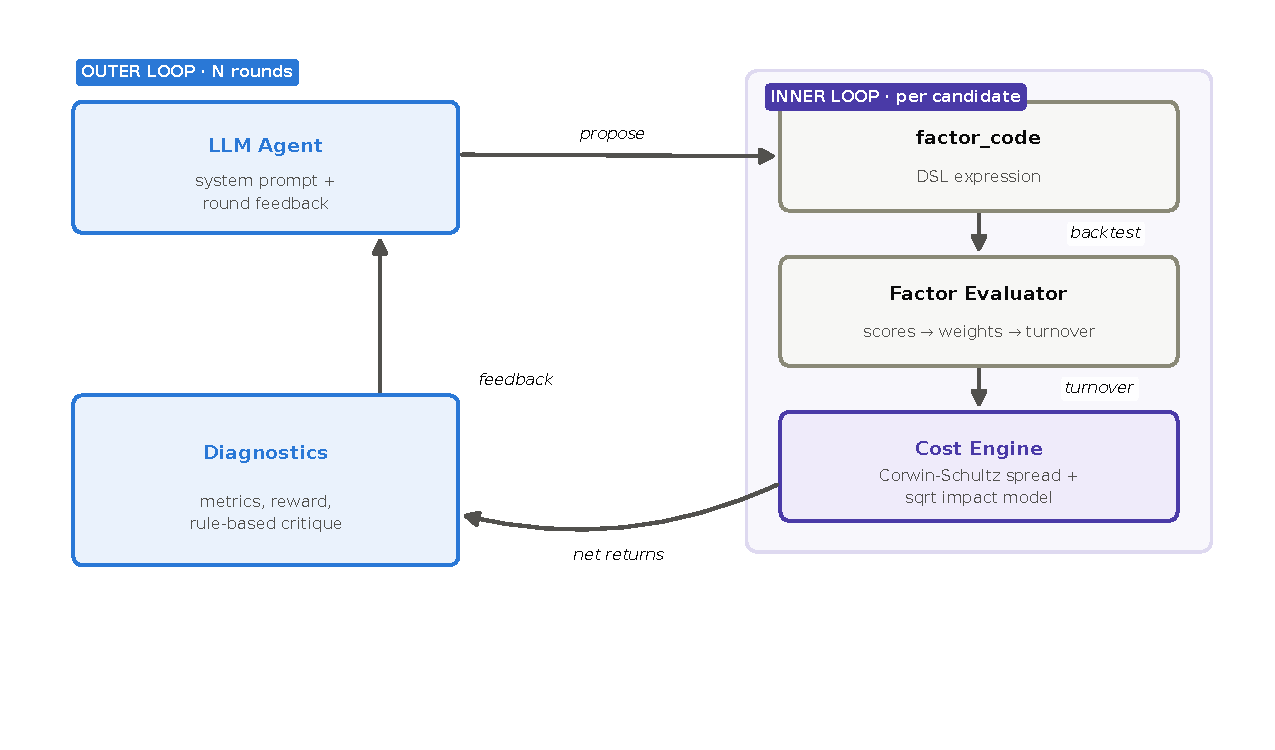
\includegraphics[width=0.85\linewidth]{figures/Figure_1.pdf}
\caption{The closed search loop. Each round the LLM agent proposes a factor expression; the evaluator turns it into dollar-neutral weights and turnover, the cost engine prices the trades, and the resulting metrics, reward and rule-based critique are returned to the agent for the next round. The three feedback conditions differ only in the reward and in the text of the reward description and critique (Table~\ref{tab:arms}).}
\label{fig:arch}
\end{figure}

\begin{table}[t]
\centering
\caption{The three feedback conditions. All arms share the system prompt, the diagnostics shown each round, the starting expression, the LLM sampling seed and the 50-round search budget.}
\label{tab:arms}
\footnotesize
\begin{tabular}{>{\raggedright\arraybackslash}p{0.19\linewidth}>{\raggedright\arraybackslash}p{0.22\linewidth}>{\raggedright\arraybackslash}p{0.22\linewidth}>{\raggedright\arraybackslash}p{0.24\linewidth}}
\toprule
 & Cost-blind & Reward-only & Execution-aware \\
\midrule
Score used to select the best factor & Gross Sharpe & Eq.~\eqref{eq:reward} & Eq.~\eqref{eq:reward} \\
\addlinespace
Reward sentence in the prompt & ``Gross Sharpe; turnover and cost are not scored'' & ``A scalar computed from the diagnostics (formula not disclosed)'' & Eq.~\eqref{eq:reward}, stating that turnover and cost are penalized, with a target of 300\% annual turnover \\
\addlinespace
Rule-based critique & Gross-return advice when gross Sharpe is weak & Same as cost-blind & Turnover above target: wrap the signal in \texttt{decay\_linear} with a longer window; large cost gap: prioritize turnover reduction \\
\bottomrule
\end{tabular}
\end{table}

\subsection{Walk-forward evaluation and inference}\label{sec:wfo}

Iterated search over many candidates scored on the same data overstates skill \citep{bailey2014}, so each search is confined to a training window and judged on data it never sees \citep{lopezdeprado2018}. Twenty-one rolling folds pair a five-year training window with the following one-year test window, rolling forward one year at a time; the test windows run from January 2006 to August 2026. In each fold and arm the agent runs 50 rounds on the training window, the best-scoring expression is frozen and the test-window returns of the 21 frozen expressions are concatenated into one 20.6-year out-of-sample record.

We seed the search with four signals from economically distinct predictor families: one-day reversal \citep{jegadeesh1990}, an abnormal-volume fade \citep{gervais2001}, low realized volatility \citep{ang2006} and volatility-scaled 60-day momentum \citep{jegadeesh1993}. Each seed is run with three LLM sampling seeds, giving 12 combinations per arm. Within a combination, the arms start from the same expression and use identically seeded but independent model instances, so they differ only in the feedback they receive.

Our main statistic is the paired difference in out-of-sample net Sharpe ratio between two arms in the same fold, combination and test year, which gives 252 fold pairs per comparison. Folds within a combination share overlapping training windows, so we resample the 12 combinations with replacement, keeping each combination's 21 folds together (10,000 cluster-bootstrap draws), to form confidence intervals and complement them with an exact sign test on the 12 combination-level mean differences.

\section{Results}\label{sec:results}

\subsection{Cost-blind versus cost-aware search}\label{sec:main}

Table~\ref{tab:main} reports each arm's stitched out-of-sample record by category, averaged across the three sampling seeds. The cost-blind arm settles on turnover of 36\% (low volatility) to 103\% (volume) of capital per day, rotating the book roughly once a day in three of the four categories, and loses its entire capital in every category. Its average gross out-of-sample Sharpe ratio is nonetheless positive (0.56; between 0.33 for volume and 0.74 for low volatility): the cost-blind search finds signals with genuine pre-cost predictive content and then trades them at a pace that costs overwhelm. Figure~\ref{fig:cum} shows the cumulative net returns for one sampling seed per category, and Figure~\ref{fig:bps} shows that the ordering of the arms holds under every flat cost assumption from 5 to 20 basis points. The figure also shows how sensitive each arm is to the cost level: raising costs from 5 to 20 basis points lowers the cost-blind arm's net Sharpe ratio by 2.5--6.6 per category, the reward-only arm's by 0.2--2.7 and the execution-aware arm's by at most 0.2.

\begin{table}[t]
\centering
\caption{Out-of-sample performance by seed signal and feedback condition, 2006--2026. Values are means across three LLM sampling seeds (standard deviation of net Sharpe in parentheses); each record stitches 21 one-year test windows.}
\label{tab:main}
\footnotesize
\resizebox{\linewidth}{!}{\begin{tabular}{llrrrrrr}
\toprule
Seed alpha & Arm & Gross SR & Net SR (s.d.) & Turnover/day & Holding (days) & Max DD & Cum. return \\
\midrule
Reversal & Cost-blind & 0.65 & $-$10.10 (0.94) & 94.9\% & 1.1 & $-$100\% & $-$100\% \\
 & Reward-only & 0.25 & $-$4.64 (1.27) & 46.0\% & 2.3 & $-$100\% & $-$100\% \\
 & Execution-aware & $-$0.03 & $-$0.28 (0.05) & 3.9\% & 26.1 & $-$82\% & $-$76\% \\
\addlinespace
Volume & Cost-blind & 0.33 & $-$11.71 (0.63) & 103.0\% & 1.0 & $-$100\% & $-$100\% \\
 & Reward-only & 0.08 & $-$2.97 (0.28) & 29.2\% & 3.5 & $-$100\% & $-$100\% \\
 & Execution-aware & 0.03 & $-$0.25 (0.03) & 3.7\% & 27.3 & $-$76\% & $-$65\% \\
\addlinespace
Volatility & Cost-blind & 0.74 & $-$3.61 (1.06) & 35.9\% & 2.9 & $-$100\% & $-$100\% \\
 & Reward-only & 0.52 & 0.25 (0.16) & 2.7\% & 37.7 & $-$34\% & +63\% \\
 & Execution-aware & 0.65 & 0.51 (0.04) & 1.4\% & 70.7 & $-$20\% & +203\% \\
\addlinespace
Momentum & Cost-blind & 0.51 & $-$7.51 (1.85) & 73.2\% & 1.4 & $-$100\% & $-$100\% \\
 & Reward-only & 0.06 & $-$0.75 (0.23) & 11.0\% & 9.2 & $-$95\% & $-$93\% \\
 & Execution-aware & 0.10 & $-$0.03 (0.05) & 1.8\% & 54.6 & $-$66\% & $-$32\% \\
\bottomrule
\end{tabular}
}
\tablenote{\emph{Notes:} Gross and net Sharpe ratios (SR) are annualized; net SR uses the full spread-and-impact cost model. Turnover is one-way daily turnover as a percentage of capital; holding period is its reciprocal in trading days. Max DD is the maximum drawdown of the net return record.}
\end{table}

The execution-aware arm cuts turnover to 1.4--3.9\% per day in every category, a 24- to 40-fold reduction, while its gross Sharpe ratio falls by much less than costs fall. The low-volatility category is the clearest case. The execution-aware arm's gross Sharpe ratio (0.65) is slightly below the cost-blind arm's (0.74), yet it is net profitable in all three sampling seeds (net Sharpe 0.48--0.56, CAGR 5.1--6.1\% at about 12\% annualized volatility, maximum drawdown $-20$\% to $-22$\%), whereas the cost-blind arm loses everything. A moderately weaker signal traded at a sustainable pace outperforms a stronger one traded at an unsustainable pace. In the other three categories the execution-aware arm loses money net of costs, but by small margins ($-0.03$ to $-0.28$) rather than the cost-blind arm's $-7.5$ to $-11.7$.

The magnitude of the cost-blind losses follows directly from the turnover. At a representative 70\% daily turnover, the book trades 140\% of capital each day across both legs; at the cost model's average of roughly 28 basis points per unit traded for these portfolios (25--29 across categories and seeds), the drag is about 0.4\% of capital per day, or roughly 100\% per year, which no gross Sharpe ratio in the range we observe can offset. The size of these losses depends on the cost level, but their sign does not. Under a flat cost of 5 basis points per unit traded, the cost-blind arm's average net Sharpe ratio is still negative in every category ($-0.11$ for low volatility to $-1.89$ for volume) and in 11 of the 12 combinations, whereas the execution-aware arm's ranges from $-0.09$ to $0.62$ (Figure~\ref{fig:bps}).

\begin{figure}[t]
\centering
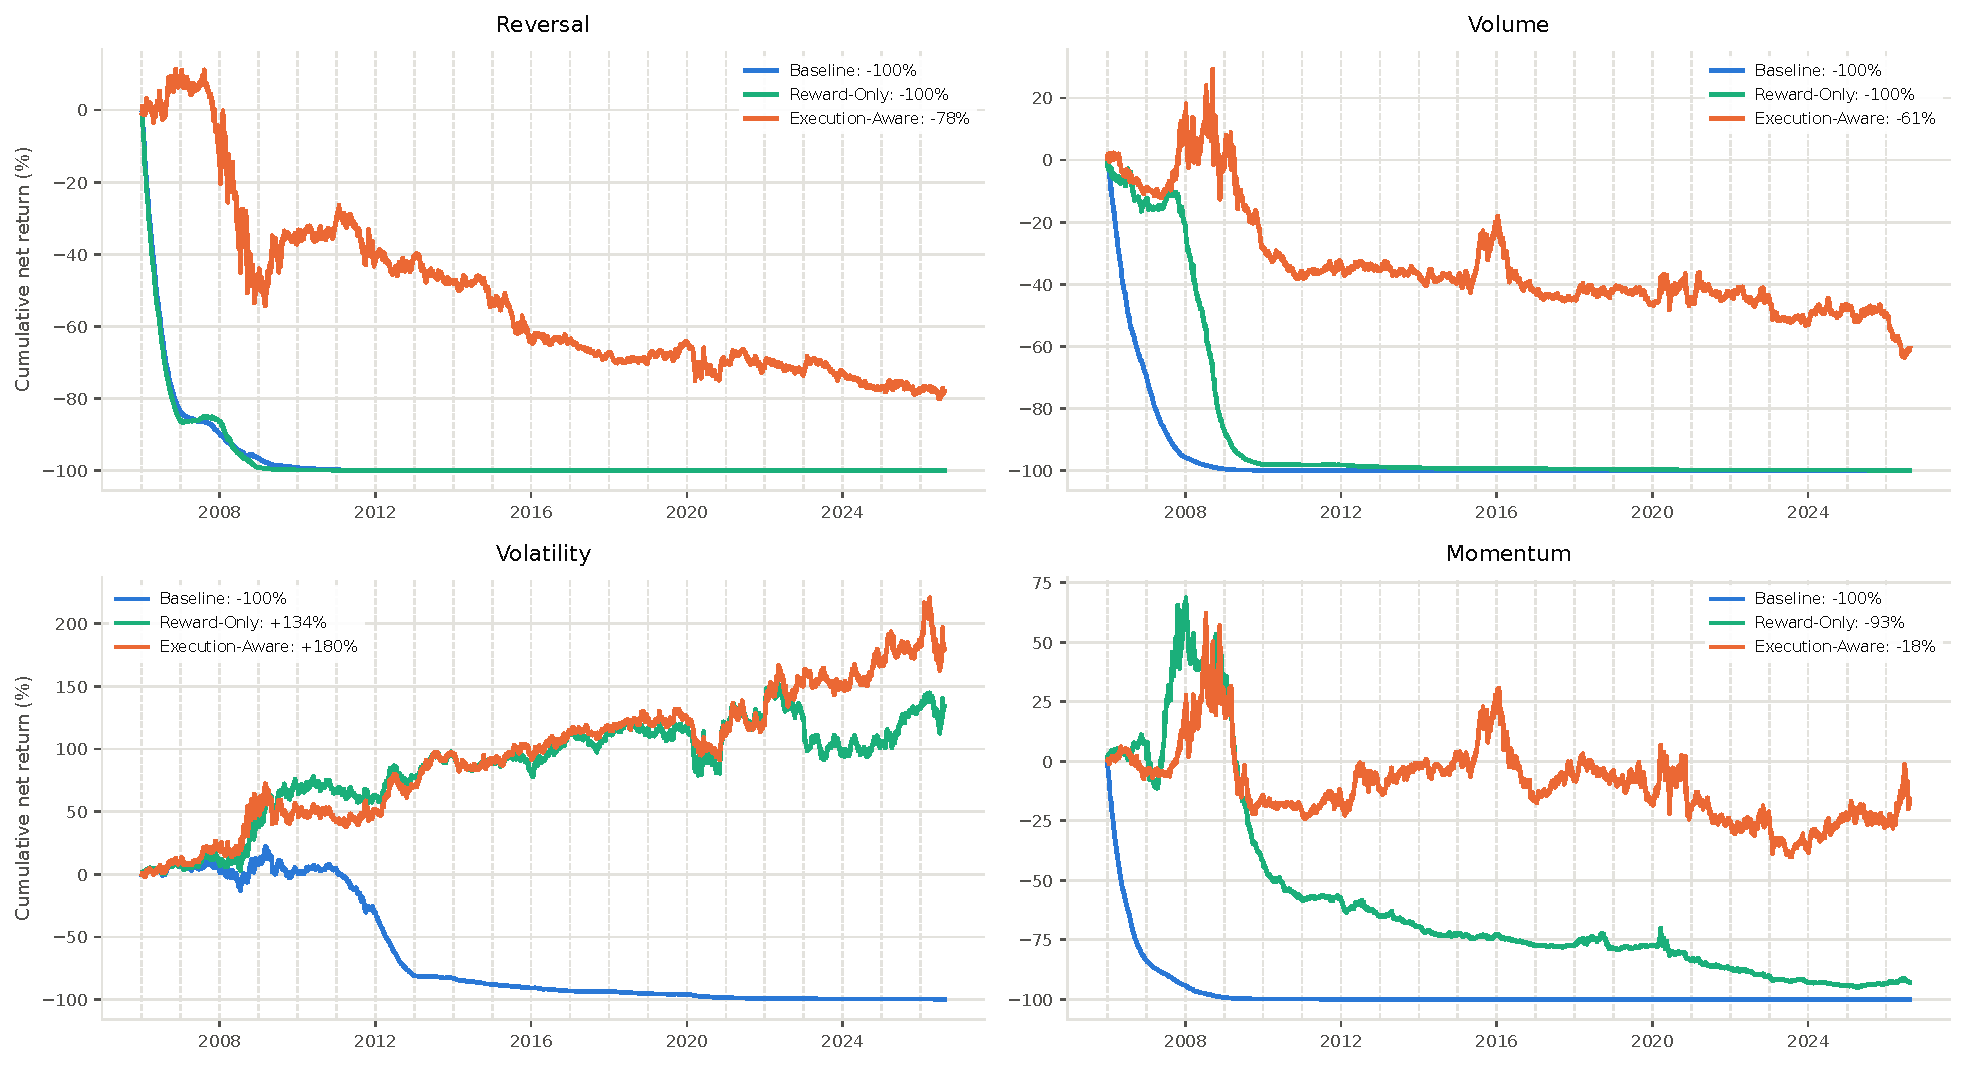
\includegraphics[width=\linewidth]{figures/Figure_2.pdf}
\caption{Cumulative out-of-sample net return. One panel per seed signal for LLM sampling seed 1001; dashed vertical lines mark the annual refit dates. Legends give the final cumulative return. Table~\ref{tab:main} reports the three-seed means.}
\label{fig:cum}
\end{figure}

\begin{figure}[t]
\centering
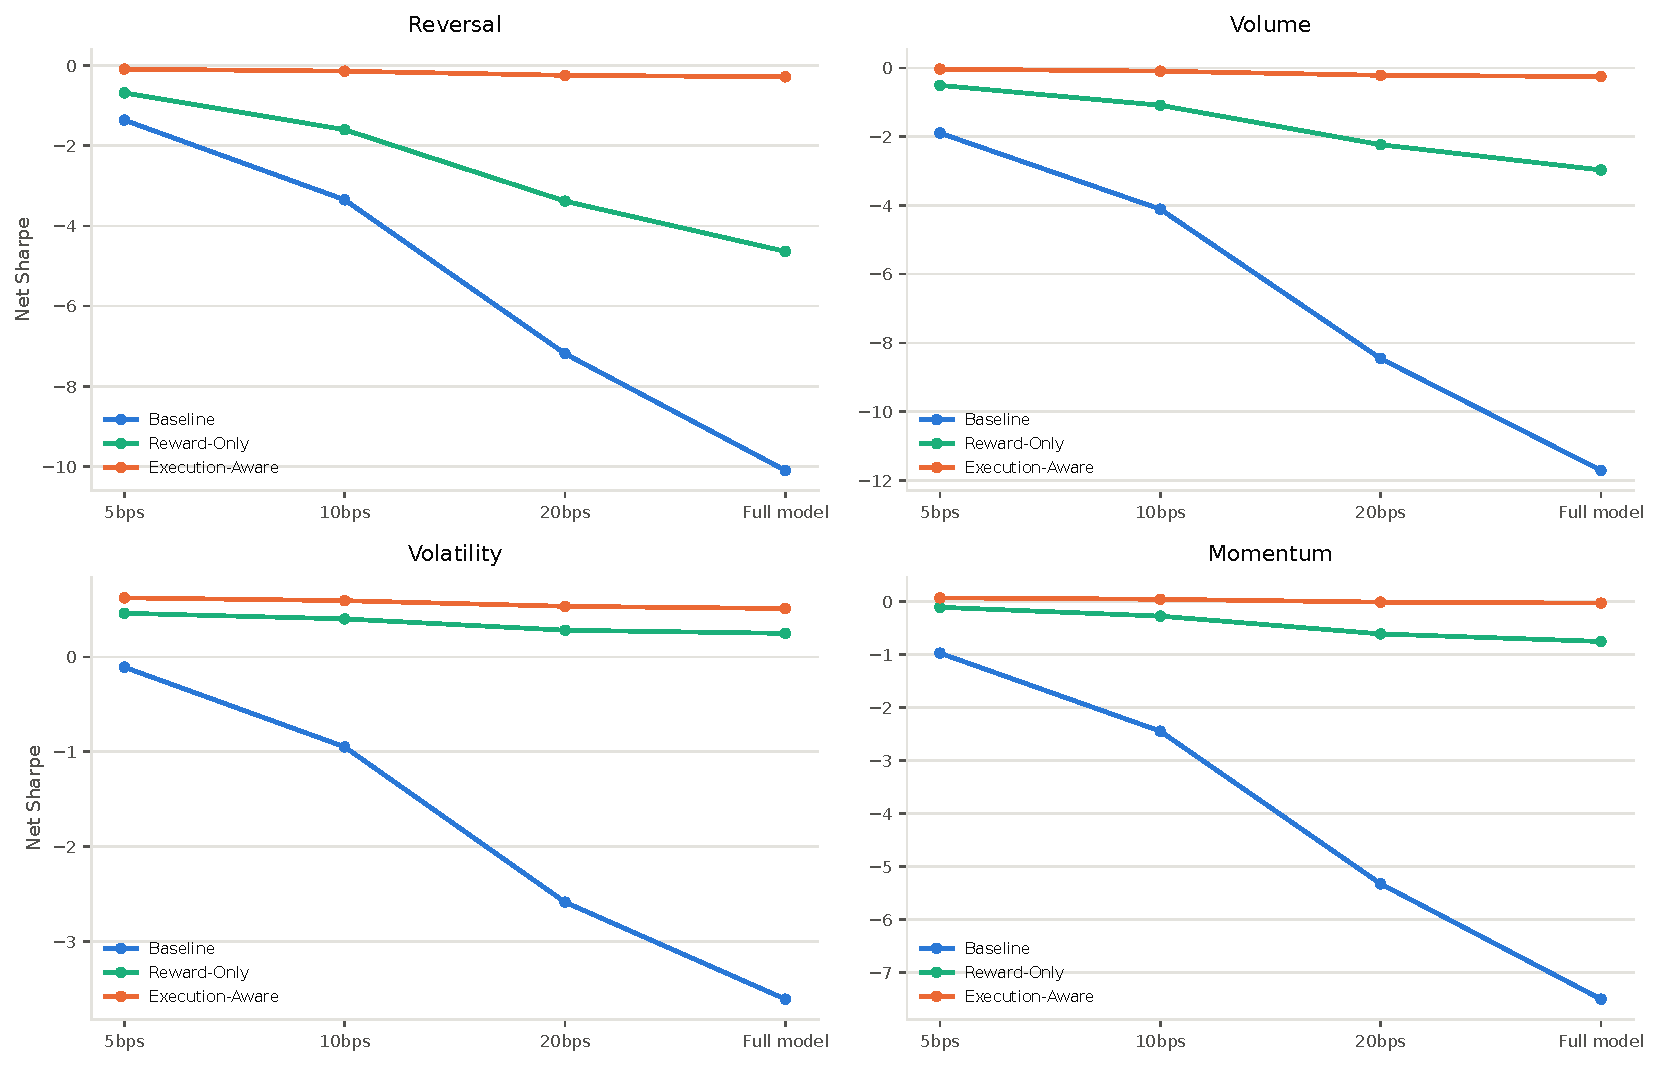
\includegraphics[width=\linewidth]{figures/Figure_3.pdf}
\caption{Net Sharpe ratio under alternative cost assumptions. Flat one-way costs of 5, 10 and 20 basis points and the full spread-and-impact model, averaged across the three LLM sampling seeds.}
\label{fig:bps}
\end{figure}

\subsection{Reward versus language}\label{sec:decomp}

Table~\ref{tab:tests} decomposes the improvement. Scoring candidates on the cost-penalized reward without explaining it raises fold-level net Sharpe by 7.9 (95\% CI 6.4--9.6) relative to the cost-blind arm, and all 12 combinations improve. These are differences between arms, not Sharpe ratios that any portfolio attains: the cost-blind arm's net Sharpe ratios run from $-3.6$ to $-11.7$ (Table~\ref{tab:main}), so most of the gain consists of pulling deeply negative ratios toward zero, and the highest net Sharpe ratio of any arm is 0.51. The reward alone therefore accounts for about three quarters of the total improvement of 10.3 (8.1--12.4). Adding the explanation, the turnover target and the cost-focused critiques adds a further 2.4 (1.3--3.7), again with all 12 combinations improving and the execution-aware arm winning 62--84\% of individual folds against the reward-only arm.

\begin{table}[t]
\centering
\caption{Paired differences in out-of-sample net Sharpe ratio between feedback conditions.}
\label{tab:tests}
\footnotesize
\resizebox{\linewidth}{!}{\begin{tabular}{lrcccrrrr}
\toprule
 & & & \multicolumn{2}{c}{Combinations} & \multicolumn{4}{c}{Folds won} \\
\cmidrule(lr){4-5}\cmidrule(lr){6-9}
Comparison & $\Delta$ Net SR & 95\% CI & positive & sign-test $p$ & Rev. & Vol. & Volat. & Mom. \\
\midrule
Reward-only $-$ cost-blind & +7.92 & [6.36, 9.56] & 12/12 & 0.0005 & 79\% & 92\% & 89\% & 89\% \\
Execution-aware $-$ reward-only & +2.42 & [1.30, 3.68] & 12/12 & 0.0005 & 78\% & 84\% & 62\% & 83\% \\
Execution-aware $-$ cost-blind & +10.34 & [8.13, 12.42] & 12/12 & 0.0005 & 87\% & 100\% & 97\% & 92\% \\
\bottomrule
\end{tabular}
}
\tablenote{\emph{Notes:} $\Delta$ Net SR is the mean paired difference over 252 fold pairs (21 folds $\times$ 12 combinations). Confidence intervals come from 10,000 cluster-bootstrap draws that resample the 12 seed-signal and sampling-seed combinations. The sign test is an exact two-sided binomial test on the 12 combination-level means. The last four columns give the share of folds in which the first arm has the higher net Sharpe ratio, by seed signal.}
\end{table}

The economic significance of the second step lies in the fast-signal categories. Without guidance, the reward-only arm still trades 46\% of capital per day in reversal and 29\% in volume and loses its entire capital in both; with guidance, turnover falls below 4\% and both categories avoid a total loss, although they still lose money net of costs (Table~\ref{tab:main}). Selection pressure alone steers an LLM agent away from the most expensive proposals, but it does not reliably lead the agent to the structural fix.

Table~\ref{tab:mechanism} shows what that fix is. Execution-aware winners use \texttt{decay\_linear} in all 252 fold instances, with an average lookback of 214 trading days, and they are simpler (6.1 operator nodes against 9.2 for the cost-blind arm). Reward-only winners use \texttt{decay\_linear} more often than cost-blind winners (62\% against 21\%) but with short windows (33 days on average), much like the cost-blind arm (28 days). The execution-aware arm's winners use much longer \texttt{decay\_linear} windows (214 days on average), and this is attributable to the guidance it receives. The execution-aware winners are also more consistent: across a category's 63 fold instances (21 folds $\times$ 3 sampling seeds), its most frequent winning expression recurs 8--21 times, against 1--5 for the cost-blind arm.

\begin{table}[t]
\centering
\caption{Structure of the winning factors (252 fold instances per arm).}
\label{tab:mechanism}
\footnotesize
\resizebox{\linewidth}{!}{\begin{tabular}{lrrrr}
\toprule
Arm & Uses \texttt{decay\_linear} & Mean lookback (days) & Mean nodes & Modal recurrences (of 63) \\
\midrule
Cost-blind & 21\% & 28 & 9.2 & 1--5 \\
Reward-only & 62\% & 33 & 8.9 & 1--13 \\
Execution-aware & 100\% & 214 & 6.1 & 8--21 \\
\bottomrule
\end{tabular}
}
\tablenote{\emph{Notes:} Lookback is the mean window parameter of a winning expression's rolling operators. Nodes counts function calls and operators. Modal recurrences is the range, across the four seed signals, of how many of the 63 fold instances share the most frequent winning expression. Table~\ref{tab:modal} lists these expressions.}
\end{table}

\subsection{What the searches converge to}\label{sec:modal}

Table~\ref{tab:modal} lists the most frequent winning expression per category and arm. The execution-aware arm turns each seed into a slow version of a related signal. One-day reversal becomes a smoothed 504-day reversal, the abnormal-volume fade a smoothed 252-day volume z-score, and 60-day momentum a smoothed, volatility-scaled 240-day momentum; the low-volatility seed is kept almost unchanged and smoothed over 240 days. The cost-blind arm rarely repeats a winner (1--5 of 63 instances) and sometimes abandons the seed's mechanism altogether: in the momentum category its most frequent winner is a volume-to-price ratio.

\begin{table}[t]
\centering
\caption{Most frequent winning expression by seed signal and feedback condition (count out of 63 fold instances).}
\label{tab:modal}
\footnotesize
\resizebox{\linewidth}{!}{\begin{tabular}{llp{0.62\textwidth}r}
\toprule
Seed alpha & Arm & Most frequent winning expression & Count \\
\midrule
Reversal & Cost-blind & \texttt{\footnotesize rank(-1 * delta(close, 1))} & 3 \\
 & Reward-only & \texttt{\footnotesize cs\_rank(-1 * ts\_rank(close, 21) + zscore(volume, 21) + sma(close, 21) - cs\_rank(high - low) + decay\_linear(vwap, 21))} & 1 \\
 & Execution-aware & \texttt{\footnotesize decay\_linear(cs\_rank(-1 * delta(close, 504)), 252)} & 8 \\
\addlinespace
Volume & Cost-blind & \texttt{\footnotesize cs\_rank(vwap - open) * cs\_rank(zscore(volume, 20))} & 1 \\
 & Reward-only & \texttt{\footnotesize cs\_rank(-1 * zscore(close, 20) + sma(vwap, 20) + decay\_linear(volume, 20))} & 1 \\
 & Execution-aware & \texttt{\footnotesize decay\_linear(cs\_rank(-1 * zscore(volume, 252)), 252)} & 14 \\
\addlinespace
Volatility & Cost-blind & \texttt{\footnotesize rank(-1 * stddev(delta(close, 1), 20) / (cs\_rank(volume) + 1e-5))} & 3 \\
 & Reward-only & \texttt{\footnotesize rank(-1 * decay\_linear(stddev(delta(close, 1), 20), 20) * cs\_rank(vwap))} & 2 \\
 & Execution-aware & \texttt{\footnotesize decay\_linear(rank(-1 * stddev(delta(close, 1), 20)), 240)} & 17 \\
\addlinespace
Momentum & Cost-blind & \texttt{\footnotesize cs\_rank(volume / (vwap + 1e-5))} & 5 \\
 & Reward-only & \texttt{\footnotesize rank(delta(close, 60) / (stddev(delta(close, 1), 60) + 1e-5))} & 13 \\
 & Execution-aware & \texttt{\footnotesize decay\_linear(cs\_rank(delta(close, 240) / (stddev(delta(close, 1), 240) + 1e-5)), 252)} & 21 \\
\bottomrule
\end{tabular}
}
\end{table}

\subsection{Sensitivity to the penalty weights}\label{sec:gamma}

Equation~\eqref{eq:reward} fixes $\gamma_1 = 0.5$ and $\gamma_2 = 8$. To check that the results do not hinge on that choice, we rerun the execution-aware arm in the low-volatility category (sampling seed 1001) with nine alternative weightings: a turnover penalty alone ($\gamma_1 \in \{0.1, 0.25, 0.5, 1\}$, $\gamma_2 = 0$), a cost penalty alone ($\gamma_1 = 0$, $\gamma_2 \in \{2, 4, 8, 16\}$) and a combined midpoint ($\gamma_1 = 0.25$, $\gamma_2 = 4$). All nine are net profitable (net Sharpe 0.29--0.52, turnover 1.4--3.3\% per day; Table~\ref{tab:gamma}). The response is a threshold rather than a smooth trade-off: any turnover penalty brings turnover down to about 1.4\% per day, after which its size barely matters, while the cost penalty alone is weaker at $\gamma_2 = 2$ and levels off from $\gamma_2 = 8$.

\begin{table}[t]
\centering
\caption{Penalty-weight sensitivity: execution-aware arm, low-volatility seed, LLM sampling seed 1001.}
\label{tab:gamma}
\footnotesize
\begin{tabular}{lrrrrrr}
\toprule
Penalty & $\gamma_1$ & $\gamma_2$ & Gross SR & Net SR & Turnover/day & Cum. return \\
\midrule
Cost-blind & 0.00 & 0 & 0.77 & $-$2.40 & 28.00\% & $-$100\% \\
Turnover only & 0.10 & 0 & 0.62 & 0.48 & 1.47\% & +181\% \\
Turnover only & 0.25 & 0 & 0.67 & 0.52 & 1.42\% & +214\% \\
Turnover only & 0.50 & 0 & 0.65 & 0.50 & 1.42\% & +199\% \\
Turnover only & 1.00 & 0 & 0.66 & 0.52 & 1.41\% & +205\% \\
Cost only & 0.00 & 2 & 0.58 & 0.29 & 3.29\% & +81\% \\
Cost only & 0.00 & 4 & 0.63 & 0.40 & 2.40\% & +134\% \\
Cost only & 0.00 & 8 & 0.65 & 0.50 & 1.57\% & +193\% \\
Cost only & 0.00 & 16 & 0.64 & 0.49 & 1.50\% & +190\% \\
Combined & 0.25 & 4 & 0.65 & 0.50 & 1.42\% & +199\% \\
Combined (main grid) & 0.50 & 8 & 0.62 & 0.48 & 1.42\% & +180\% \\
\bottomrule
\end{tabular}

\tablenote{\emph{Notes:} The first and last rows are the cost-blind and execution-aware arms of the main experiment for the same seed signal and sampling seed. Turnover is one-way daily turnover as a percentage of capital.}
\end{table}

\subsection{Is the search necessary?}\label{sec:controls}

A natural question is whether an LLM search is needed at all: perhaps the seed signal, slowed down by a simple rule, does as well. Table~\ref{tab:controls} compares the two cost-aware arms with four rules that use no search, scored on the same folds, universes and cost model: the seed signal rebalanced daily, the seed signal rebalanced every 21 trading days, the seed signal smoothed with \texttt{decay\_linear} over 252 days and the cost-blind arm's winning factors rebalanced every 21 trading days.

\begin{table}[t]
\centering
\caption{Comparison with rules that use no search: out-of-sample net Sharpe ratio (Net SR) and daily turnover (TO), 2006--2026.}
\label{tab:controls}
\footnotesize
\resizebox{\linewidth}{!}{\begin{tabular}{lrrrrrrrr}
\toprule
 & \multicolumn{2}{c}{Reversal} & \multicolumn{2}{c}{Volume} & \multicolumn{2}{c}{Volatility} & \multicolumn{2}{c}{Momentum} \\
\cmidrule(lr){2-3}\cmidrule(lr){4-5}\cmidrule(lr){6-7}\cmidrule(lr){8-9}
Strategy & Net SR & TO/day & Net SR & TO/day & Net SR & TO/day & Net SR & TO/day \\
\midrule
Seed alpha, daily & $-$14.00 & 128.5\% & $-$14.17 & 96.6\% & 0.00 & 6.6\% & $-$1.26 & 16.5\% \\
Seed alpha, monthly & $-$0.56 & 6.1\% & $-$1.14 & 6.6\% & 0.48 & 1.9\% & $-$0.42 & 3.7\% \\
\texttt{decay\_linear}(seed, 252), daily & $-$0.60 & 10.9\% & $-$1.21 & 12.6\% & 0.48 & 1.4\% & $-$0.10 & 2.3\% \\
Cost-blind winners, monthly & $-$0.36 & 5.2\% & $-$0.63 & 5.8\% & 0.17 & 3.1\% & $-$0.17 & 4.5\% \\
\midrule
Reward-only search & $-$4.64 & 46.0\% & $-$2.97 & 29.2\% & 0.25 & 2.7\% & $-$0.75 & 11.0\% \\
Execution-aware search & $-$0.28 & 3.9\% & $-$0.25 & 3.7\% & 0.51 & 1.4\% & $-$0.03 & 1.8\% \\
\bottomrule
\end{tabular}
}
\tablenote{\emph{Notes:} Monthly rules trade to their target weights every 21 trading days and let positions drift in between. The cost-blind winners are each fold's frozen cost-blind factor, averaged across the three sampling seeds. The smoothing window of 252 days and the monthly frequency were chosen after observing the execution-aware results, which favors these rules.}
\end{table}

Three results stand out. First, in three of the four categories the execution-aware search is close to the best rule. In low volatility the seed alone breaks even (net Sharpe 0.00), while smoothing it or rebalancing it monthly yields 0.48 against the search's 0.51; in reversal and momentum the search leads the best rule by 0.08 and 0.07 ($-0.28$ against $-0.36$, and $-0.03$ against $-0.10$). Only in volume is the gap large ($-0.25$ against $-0.63$). Second, in some categories the search does more than slow the seed down: in reversal and volume its winners also lengthen the signal's own horizon (from one-day to 504-day reversal, and from a 20-day to a 252-day volume z-score), In low volatility, by contrast, it only slows the seed down: its most frequent winner is the seed itself, smoothed. Third, rebalancing the cost-blind winners monthly recovers most of their losses but still falls short of the execution-aware arm in all four categories, and it has two drawbacks. It adds settings that must be chosen outside the search, such as the rebalancing frequency or the smoothing window, whereas the execution-aware search chooses its horizon itself. And those winners were selected for their short-horizon predictive power with costs ignored, so much of that power has faded by the time a monthly trade is made.

The rules here use conventional settings (a one-year smoothing window and monthly rebalancing) without tuning. Choosing these settings fold by fold from training data, as the search chooses its horizons, is left for future work.

\subsection{Factor exposures}\label{sec:spanning}

Table~\ref{tab:spanning} regresses each arm's daily net returns, averaged across the three sampling seeds, on the \citet{fama2015} five factors and momentum \citep{carhart1997,french2026}, with \citet{newey1987} standard errors (five lags). In the low-volatility category, the execution-aware arm earns an alpha of 7.8\% per year ($t = 3.48$) with the exposures expected of a low-volatility portfolio: a negative market beta and positive loadings on profitability (RMW) and investment (CMA). For comparison, the two rules built directly from the seed (monthly rebalancing and 252-day smoothing; Section~\ref{sec:controls}) have nearly identical alphas (7.3--7.7\% per year) and loadings, so the search and the rules capture the same low-volatility premium. In the other three categories, the execution-aware arm's alphas are not statistically different from zero at the 5\% level, and its returns load heavily on momentum: positively for the momentum seed (loading 0.72, $R^2 = 0.72$) and the volume seed (0.45), and negatively for the reversal seed ($-0.62$), whose 504-day reversal is close to a negative momentum position.

\begin{table}[t]
\centering
\caption{Factor regressions of daily out-of-sample net returns, 2006--2026.}
\label{tab:spanning}
\footnotesize
\resizebox{\linewidth}{!}{\begin{tabular}{lrrrrrrrrr}
\toprule
Strategy & $\alpha$ (\%/yr) & ($t$) & Mkt & SMB & HML & RMW & CMA & Mom & $R^2$ \\
\midrule
Reversal: cost-blind & $-$128.1 & ($-$50.60) & 0.05 & 0.01 & 0.06 & $-$0.07 & $-$0.06 & 0.00 & 0.02 \\
Reversal: reward-only & $-$61.7 & ($-$30.12) & 0.01 & $-$0.05 & 0.12 & $-$0.12 & $-$0.12 & $-$0.04 & 0.06 \\
Reversal: execution-aware & $-$4.9 & ($-$1.91) & 0.12 & 0.02 & 0.20 & $-$0.16 & 0.17 & $-$0.62 & 0.57 \\
\addlinespace
Volume: cost-blind & $-$144.0 & ($-$71.13) & 0.03 & 0.01 & 0.11 & $-$0.08 & $-$0.11 & 0.02 & 0.04 \\
Volume: reward-only & $-$38.9 & ($-$18.98) & 0.01 & 0.01 & 0.00 & $-$0.01 & $-$0.09 & $-$0.03 & 0.02 \\
Volume: execution-aware & $-$4.3 & ($-$1.67) & $-$0.08 & 0.11 & $-$0.20 & 0.09 & 0.16 & 0.45 & 0.41 \\
\addlinespace
Volatility: cost-blind & $-$39.4 & ($-$18.40) & $-$0.09 & 0.12 & 0.10 & 0.02 & 0.23 & $-$0.05 & 0.14 \\
Volatility: reward-only & +3.9 & (1.97) & $-$0.09 & 0.08 & 0.05 & 0.09 & 0.23 & $-$0.14 & 0.16 \\
Volatility: execution-aware & +7.8 & (3.48) & $-$0.22 & 0.14 & 0.04 & 0.21 & 0.40 & 0.04 & 0.27 \\
\addlinespace
Momentum: cost-blind & $-$98.3 & ($-$37.73) & 0.02 & 0.05 & $-$0.05 & $-$0.10 & 0.02 & 0.08 & 0.04 \\
Momentum: reward-only & $-$12.2 & ($-$5.20) & $-$0.11 & 0.06 & $-$0.16 & 0.13 & 0.14 & 0.30 & 0.30 \\
Momentum: execution-aware & $-$1.8 & ($-$0.98) & $-$0.02 & $-$0.17 & $-$0.07 & 0.06 & $-$0.17 & 0.72 & 0.72 \\
\midrule
Volatility: seed, monthly & +7.3 & (3.42) & $-$0.21 & 0.12 & 0.05 & 0.18 & 0.38 & $-$0.09 & 0.26 \\
Volatility: \texttt{decay\_linear}(seed, 252) & +7.7 & (3.43) & $-$0.23 & 0.16 & 0.04 & 0.21 & 0.42 & 0.01 & 0.28 \\
\bottomrule
\end{tabular}
}
\tablenote{\emph{Notes:} Daily net returns of each arm are averaged across the three LLM sampling seeds and regressed on the Fama--French five factors and the momentum factor. $\alpha$ is the annualized intercept (daily intercept $\times$ 252); $t$-statistics use Newey--West standard errors with five lags. The cost-blind alphas are large and negative because those strategies lose their capital through trading costs.}
\end{table}

\section{Discussion and limitations}\label{sec:discussion}

A reward that penalizes turnover will, mechanically, select lower-turnover factors. The substantive question is whether the trade-off improves realized out-of-sample performance, and the evidence says it does: turnover falls by more than an order of magnitude, gross Sharpe falls much less, net Sharpe improves in every combination and the improvement survives every penalty weighting we test. The decomposition adds a less obvious point. An LLM agent responds to a reward it is shown as a number, but it responds more effectively when the objective is spelled out and paired with targeted feedback. For practitioners building such agents, this means that the prompt and critique are part of the objective, and should be reported alongside it.

Several limitations qualify these results. The execution-aware critique explicitly recommends longer smoothing windows, so the structural convergence in Table~\ref{tab:mechanism} reflects guidance rather than unaided discovery; the reward-only arm measures how far the model gets without it. The reward-only arm's prompt differs from the cost-blind arm's in its reward sentence as well as its scores, so the first step of the decomposition combines selection pressure with a neutral description of the objective. All runs use one open-weight model at one quantization and temperature, so the magnitudes may differ for other models. The penalty-weight sweep covers one category and one sampling seed. Each fold trades the 150 most liquid constituents rather than the full index, and the impact coefficient is a textbook value rather than an estimate from execution data; the flat-cost results show that the ranking of the arms does not depend on the cost level, but they share the cost model's functional form. Portfolio construction is deliberately unconstrained (daily rebalancing at 200\% gross exposure with no trading band), which makes the cost channel and the agent's response to it visible, and makes the negative net Sharpe ratios in three categories a stress test rather than evidence that these predictor families cannot be traded profitably. Finally, Sharadar does not provide delisting returns, so the last traded price before a delisting is the final observation.

\section{Conclusion}\label{sec:conclusion}

Holding the search procedure, model, data and cost model fixed and varying only the feedback, a locally hosted LLM factor-mining agent rewarded on gross returns settles on daily turnover of 36--103\% and loses its entire capital in all four seed categories, despite positive average gross Sharpe ratios. Scoring the same search on a cost-penalized reward raises fold-level net Sharpe by 7.9 points, mostly by pulling deeply negative ratios toward zero; explaining that reward and critiquing proposals in cost terms adds a further 2.4, cuts turnover to 1.4--3.9\% per day and leads the agent to long-horizon smoothed signals. One category becomes profitable, with a factor-adjusted alpha that simple slowing rules match. The objective of an automated factor search, and the way it is communicated to an LLM agent, determines whether the search creates or destroys value net of costs.

\section*{Data availability}

The point-in-time price and membership data are licensed from Nasdaq Data Link (Sharadar) and cannot be redistributed; the Fama--French factors are publicly available from Kenneth French's data library. All code, the prompts, the full search logs, per-fold winning expressions and out-of-sample return series for every arm, and the scripts that produce every table and figure are available in a public code repository; its URL is given on the title page and withheld from this version to preserve anonymity during review.

\section*{Funding}

This research did not receive any specific grant from funding agencies in the public, commercial, or not-for-profit sectors.

\section*{Declaration of generative AI and AI-assisted technologies in the manuscript preparation process}

During the preparation of this work the author used Claude (Anthropic) to assist with drafting, editing and structuring the manuscript text, and with writing and debugging the analysis and figure-generation code. All experimental design, code execution, results and interpretations are the author's own. After using this tool, the author reviewed and edited the content as needed and takes full responsibility for the content of the published article.

\bibliographystyle{elsarticle-harv}
\bibliography{references}

\appendix

\section{Methodological details}\label{app:methods}

\subsection{Universe construction}\label{app:universe}

The Sharadar SP500 table records each addition to and removal from the index with its effective date. A stock is treated as a member from its addition date (inclusive) until its next removal date (exclusive). On each of the 114 quarter-ends from 1998 to 2026 for which Sharadar also publishes a full constituent list, this event-based membership matches the list exactly. Prices come from the Sharadar SEP table: \texttt{close} is split-adjusted, \texttt{closeadj} is adjusted for splits and dividends, and we multiply open, high and low by \texttt{closeadj}/\texttt{close} so that all prices are on a total-return basis. Sharadar fills non-trading days with the previous close and zero volume; we treat such days as missing.

For each fold, at the start of each training year and at the start of the test year, we rank the stocks that are index members on that date by their average dollar volume over the preceding 504 trading days, computed only over days on which each stock was a member, and keep the top 150. A stock is tradable on a given day only if it is an index member and belongs to the most recent annual selection.

\subsection{Expression language and guardrails}\label{app:guardrails}

The whitelist contains cross-sectional rank (\texttt{cs\_rank}, \texttt{rank}), time-series rank (\texttt{ts\_rank}), rolling z-score (\texttt{zscore}), \texttt{decay\_linear}, simple moving average (\texttt{sma}), rolling standard deviation (\texttt{stddev}), differences and lags (\texttt{delta}, \texttt{delay}), absolute value and the four arithmetic operators. Beyond the whitelist, six rules reject a candidate before any backtest: (i) a rank applied directly to a rank of the same kind; (ii) a positive constant added to or multiplied onto the whole expression, which leaves cross-sectional ranks unchanged (sign flips are allowed); (iii) more than one smoothing operator nested directly; (iv) division by a denominator that is neither protected by a small constant nor itself a rank; (v) exponents above two; and (vi) rolling windows outside 2--252 trading days (\texttt{delta} and \texttt{delay} are exempt).

\subsection{LLM settings}\label{app:llm}

The model is Qwen2.5-Coder-14B-Instruct in the Q4\_K\_M GGUF quantization, run with llama.cpp on a single GPU per arm, with a 4,096-token context, temperature 0.7, nucleus sampling at 0.9 and at most 400 output tokens per round. The agent must return a JSON object containing one expression and a one-sentence rationale; malformed or rejected proposals score negative infinity and are reported back to the agent as failures. In pilot runs on an earlier data set, complete 25- to 50-round trajectories at temperatures 0 and 0.3 settled on a fixed proposal after one or two rounds and made no further progress, so we use 0.7 and characterize sampling variation with three seeds (1001, 2002 and 3003). Within a combination, each arm uses its own model instance with the same seed; because each instance sees only its own prompts, the arms can be run in parallel without changing their outputs.

\subsection{Turnover and cost}\label{app:turnover}

Let $w_{i,t}$ be the target weight of stock $i$ formed at the close of day $t$ and $r_{i,t+1}$ its return over the next day. Before rebalancing on day $t+1$, yesterday's book has drifted to $\tilde w_{i,t+1} = w_{i,t}(1+r_{i,t+1}) / \sum_j |w_{j,t}(1+r_{j,t+1})| \times 2$, preserving 200\% gross exposure. The trade on day $t+1$ is $\Delta_{i,t+1} = w_{i,t+1} - \tilde w_{i,t+1}$; one-way turnover is $\tfrac{1}{2}\sum_i |\Delta_{i,t+1}|$, and the cost of the day is $\sum_i c_{i,t+1}\,|\Delta_{i,t+1}|$, where $c$ is the per-stock one-way cost of Section~\ref{sec:costs}. In the reward, turnover and cost are annualized by multiplying their daily means over the training window by 252.

\end{document}
